\documentclass[11pt]{article}
\usepackage[utf8]{inputenc}

\title{Qualifying Examination Paper}
\author{John Stein (jodstein@iu.edu)}
\date{November 2018}

\usepackage{natbib}
\usepackage{graphicx}
\usepackage{setspace}\singlespacing
\usepackage[left=1in, right=1in, top=1in, bottom=1in]{geometry}
\usepackage{appendix}
\usepackage{amsmath}
\usepackage{tikz}
\usetikzlibrary{positioning, shapes, arrows}
\usepackage[ruled]{algorithm2e}

\begin{document}

\begin{titlepage}
    % https://stackoverflow.com/questions/3141702/vertically-centering-a-title-page
    \null
    \nointerlineskip
    \vfill
    \let\snewpage \newpage
    \let\newpage \relax
    \maketitle
    \let \newpage \snewpage
    \vfill
    \thispagestyle{empty}
\end{titlepage}


\tableofcontents
\thispagestyle{empty}


%%%%%%%%%%%%%%%%% Paper %%%%%%%%%%%%%%%%%%%%%%
\newpage
\setcounter{page}{1}
\section{Generative Adversarial Networks (GANs)}

%\subsection{Introduction}
The Generative Adversarial Nets (GAN) framework was first introduced by Goodfellow et al. in 2014 \cite{NIPS2014_5423}.  The GAN framework involves the simultaneous training of both a generative model $G$ with parameters $\theta_g$ and a discriminative model $D$ with parameters $\theta_d$.  Given a target data space $T$ with distribution $p_t$, $G$'s task is to learn a mapping from a noisy input $z$ to the data space $T$ ($G:Z \rightarrow G(z) \sim p_g \approx p_t$); while $D$'s task is to discriminate whether some input $x$ originated from either $T$ or $G(z)$ ($D: X \rightarrow \{0, 1\}$).  Since $G$ would like to generate samples that are representative of $T$, and therefore make $D$'s task more difficult by capturing $p_t$ with $p_g$, $G$ includes a loss term that is based on whether $D$ successfully discriminated inputs as $T$ or $G(z)$ and back-propagates $D$'s success as error to $\theta_g$ appropriately.  In this way, $G$ learns how to generate data that is hard for an ever-improving $D$ to distinguish.  Importantly, labeled data is not required for either $G$ or $D$ because the loss function used by $G$ is defined in terms of $D(x)$ and $(1-D(G(z))) \in \{0, 1\}$ (ie. did $G$ fool $D$?) and the labels for $x$ essentially map to $\{p_t, p_g\}$ (ie. from target or generated data?).  Thus, the GAN framework presents a promising approach for generating data that approximates a target distribution in an unsupervised manner.

\subsection{GANs in Computer Vision}

The GAN framework has resulted in significant advancement within many Computer Vision related areas of study, and has inspired many GAN variations that represent improvements or specialized implementations.

\subsubsection{GAN Implementation Advancements}

In the original GAN, $G$ learns to generate data that estimates $p_t$, but cannot target specific sub-distributions within $p_t$, such as class labels or modes within $p_t$.  Shortly after the original GAN was introduced, Mirza and Osindero introduced an extension called Conditional GAN \cite{mirza2014conditional} which addresses this need.  By adding a conditioning input layer to both models $G$ and $D$, one can present the conditioning data $y$ alongside the normal data.  $G$ will learn a mapping from $z$ to $X$ given $y$ that will result in making classification of $X$ given $y$ difficult for $D$.  This advancement seems obvious in retrospect, but warrants contemplation.  While $G$ represents a mapping that captures the distribution of the target data space $T$ in general, the noisy input $z$ can be regarded as the diversity component of the input and $y$ can regarded as the specification component of the input.  Since $y$ is constant within a given mode, a smaller portion of the overall networks for $G$ and $D$ can focus on the generation and discrimination, respectively, of the modal contribution whereas the remaining portions of the networks can focus on the unspecified contributions from $z$.  Of course, Conditional GAN requires that conditioning data (eg. labels) are available for all target samples $x \in X$.

Radford, Metz, and Chintala \cite{DBLP:journals/corr/RadfordMC15} evaluated various model architectures and recommended a set of guidelines and constraints for $G$ and $D$ architectures that appeared to perform well in terms of stability, convergence, resolution, and depth of representation.  These guidelines describe a Deep Convolutional GAN (DCGAN) and are summarized as follows: (a) use convolution and fractional convolution layers with striding to achieve adaptive down-sampling ($D$) or up-sampling ($G$), respectively, rather than fixed/deterministic methods (i.e. max pooling), (b) use batch normalization between convolution layers to mitigate collapse or failure due to poor initialization or vanishing gradients, (c) avoid fully-connected layers, with the exception of the input to $G$ and the output of $D$, to help earlier convergence, and (d) use Rectifier Linear Unit (ReLU) activation for input and hidden layers in $G$, tanh for the output layer in $G$, and Leaky ReLU for all layers in $D$.  In addition to performance improvements, the authors demonstrate that $D$ is able to learn semantically-relevant features that are both explainable (via latent-space walk based validation) and usable (via feature-based supervised classification).  In one case they were able to discover a linear vector in $Z$-space that could control rotation of faces.  


\subsubsection{GAN in Semantic Learning and Generation}

Within the theme of semantic learning and generation, Pathak, Krahenbuhl, Donahue, Darrell, and Efros used an adversarial approach to inpaint (fill in missing portions of) images with large extents of missing pixel data \cite{pathakCVPR16context}.  Their architecture is based on an auto-encoder \cite{hinton2006reducing} combined with GAN.  In their approach, the encoder-decoder learns a semantic encoding based on the non-missing portions and attempts to reproduce a whole image based on that semantic encoding.  The `reconstruction loss' is defined in terms of distance ($L_2$) from the filled area to the removed area. The encoder-decoder is regarded as $G$, and a new discriminator $D$ is trained to predict whether its input is a reconstructed output from $G$ or an original image.  Interestingly, and in contrast with \cite{mirza2014conditional}, the authors achieved better results when $G$, but not $D$, was conditioned with context information \footnote{The paper defines context information as the missing pixels which, if true, undermines the objective (any statement of success should be based on withholding the missing pixels from the architecture).  I have requested clarification on this from the author (17 Oct 2018).}.

%Wu et al. took a somewhat similar approach and extended a variational autoencoder \cite{larsen2015autoencoding} within a 3-dimensional GAN architecture (3D-VAE-GAN) which learns to generate 3D images from 2D examples \cite{NIPS2016_6096}.

Luc, Couprie, Chintala and Verbeek applied a straightforward GAN approach to the task of semantic segmentation on images \cite{Luc2016SemanticSU}.  Their approach uses a Convolutional Neural Network (CNN) based generative model $G$ to learn a class label for each pixel in the image based on a ground-truth labeling (supervised), thereby creating a segmentation map of the input image.  $D$ then takes a segmentation map and tries to classify it as being a ground truth map or a generated map.  
%While $D$'s objective function tries to maximize classification accuracy of the input segmentation map as being either ground truth or generated, $G$'s objective function tries to maximize pixel class labeling accuracy with respect to ground truth while also minimizing accuracy.

%Ehsani, Mottaghi, and Farhadi used a GAN approach to address the related dual purpose task of semantically segmenting objects within an image and completing those objects that were occluded by other objects in the image \cite{ehsani2017segan}.

Reed et al. applied a GAN approach to the dual-task of (1) generating realistic images (2) from text-based descriptions \cite{reed2016generative}.  Essentially, they create $G$ by concatenating the input noise with an encoding of the text description and feed the result into a feed-forward CNN using fractional-striding\footnote{The paper claims this to be a de-convolutional network, but I presume it to mean a CNN using fractional striding to achieve up-sampling.}.  $D$ then down-samples with CNN layers until a 4x4 representation is achieved, concatenates the text encoding onto each of the 16 frames, and continues convolutions to achieve the binary discriminator output.  The learning objectives are consistent with \cite{NIPS2014_5423}.  However, since there are two sources of error (error associated with producing fake-looking images and error associated with producing real-looking images that do not match the description), their approach addresses the second source of error by augmenting the labeled data with real images having non-matching descriptions, which $D$ must learn to recognize.

\subsubsection{Image Translation}

Another rich area of research that has greatly benefited from the GAN architecture is image translation.  Generally, image translation deals with the learning of a meaningful semantic representation of an image in one domain, and then generating an image with the same semantic representation from a different domain.  Isola, Zhu, Zhou, and Efros designed a solution that appears to generalize well across various domain pairs for this task \cite{isola2017image}.  Their architecture follows a U-Net auto-encoder architecture \cite{ronneberger2015u} with DCGAN constraints \cite{salimans2016improved}.  Further, similar to \cite{pathakCVPR16context}, they constrain $D$'s task to focusing on high-frequency semantic accuracy using learned image patch losses that are fed from skipped connections from encoder layers (PatchGAN), while leveraging an $L_1$ term in $G$'s loss to ensure low-frequency accuracy.  A later paper from Liu, Breuel, and Kautz also displays impressive results \cite{NIPS2017_6672} in image translation.

\subsubsection{Video Implementations}

A logical step forwards from image-based applications is to apply GAN to video.  Mathieu, Couprie, and LeCun first adopted a GAN approach to a video prediction task \cite{Mathieu2015DeepMV}.  They designed a scaled generator $G_k$ that convolves input frames at scale $k$ and predicts a future frame at that scale $Y_k$.  The overall generator $G$ then generates the final predicted frame $Y$ at full resolution using a Laplacian pyramid \cite{denton2015deep} built on each $G_k$.  The discriminator $D$ attempts to classify the last frame(s) in a frame sequence as being either real or generated by $G$ (the first frames in the input sequence are always real), and thus provides the usable adversarial loss to $G$.

Tulyakov, Liu, Yang, and Kautz introduce a method for decomposing video into content (the objects in the video) and motion (the movement of those objects) components, each having its own generator and discriminator ($G_C, G_M, D_C, D_M$) \cite{tulyakov2017mocogan}.  $D_C$ attempts to detect whether a frame is sampled from a real video clip or a generated one, while $D_M$ attempts to detect whether a video clip (series of frames) is sampled from a real or generated clip.  $G_C$ (a CNN) takes motion vectors from $G_M$ (a Recurrent Neural Network), and it's objective includes loss terms from both $D_C$ (a CNN) and $D_M$ (a spatio-temporal CNN), while $G_M$'s objective includes a loss term from $D_M$ only.  In this way, the noise input to $G_C$ can control which objects are in the video, while the noise input to $G_M$ can control the objects' motion.  Another notable application involves segmentation-map-to-video synthesis \cite{wang2018videotovideo}.

%Bansal et al. tackle the task of video-to-video translation and achieve fairly convincing results with a hierarchical GAN approach (RecycleGAN) \cite{bansal2018recyclegan}.  Their approach does not require matched video pairs (between domains), but instead introduces loss terms related to reconstruction (accuracy in translating from domain A to domain B and back to domain A again), next frame prediction, and straightforward generative and aversarial losses.

\subsubsection{Implications to Security}

Like any powerful technology, there are significant security implications associated with GANs, both with respect to how they are implemented and how they are used.  Indeed, most of the papers involving GAN implementations for computer vision applications rely on the ability of generated image/video to fool a human observer as an important qualitative measure of success.  The use of deep learning as a tool for generating convincing, non-authentic video was put in the public eye when a tool set developed by deepfake \cite{deepfakes-faceswap} was used maliciously to produce pornographic video content with public personalities, and later by celebrity Jordan Peele as a public service announcement, warning of the dangers of misuse of the technology \cite{peeleDeepFakes}.  

Although this paper has only discussed the use of GANs to achieve a singular objective, learning and/or generative models can be juxtaposed by two owners with opposing goals.  Szegedy et al. introduced this as a potential issue, showing how minimally-perturbed examples can be generated which result in miss-classification (with high confidence) by a classification model.  Several follow-up studies have explored this phenomena further \cite{carlini2016towards, kos2017adversarial, moosavi2017universal, athalye2017synthesizing}, noting potentially serious consequences for applications such as robotics, autonomous vehicles, and military.

%Lastly, Shokri et al. developed an adversarial methodology for determining whether a given sample was specifically included in the training set (which, in many cases, may be considered private) for a given classification model \cite{shokri2017membership}.  Song et al. developed a methodology

\subsubsection{Remaining Challenges and Opportunities}

As discussed, the GAN approach has enabled major improvements to several research areas including semi-supervised and unsupervised learning, generative models, the learning of complex loss functions, data synthesis for other learning tasks, image and domain learning and translation, and semantic learning and generation.  In general, the GAN approach provides a relatively simple and tractable way of isolating deep learning objectives and sources of error in such a way that they can be addressed individually and researchers can make headway toward a complex objective, as is apparent in the Conditional GAN, in-painting, MoCoGAN, and text-to-image generation, among others.  Broadly stated, as deep learning models adopt more complex architectures and greater capacity, there is an increasing need to provide more meaningful and comprehensive constraint to the model's objective.  GANs provide a tractable methodology for learning sets of constraints which can be as complex as the main learning objective, or even more-so.

To this end, I predict that a likely trend in GAN research is the emergence of more complex GAN architectures.  Subdividing complex goals into multiple generators and complex constraints into multiple discriminators is likely to lead to elegant solutions to tasks previously considered to be too complex for more conventional singular deep learning models.  Likewise, as GAN architectures grow in complexity, the overall objective function (combination of loss terms, heuristics, and discriminator outputs) for a complex learning task may become a focus of future work.  Whereas, for example, current research is learning semantic representations in videos that involve specific objects and their spatial movement across several frames, deeper semantic learning of \textit{who, what, where, when, and why} information may demand these more complex hierarchical structures.

Further, as research yields models and approaches that efficiently and effectively solve moderately complex tasks, it is reasonable to expect growing a demand for standardized, modular, and extensible model interfaces (eg. Model Based Engineering ecosystem) for use among research and commercial entities to solve more complex tasks and continue the evolution of artificial intelligence.

In the area of security, GAN approaches pose both a threat (fake video, adversarial examples) as well as a benefit (eg. efficient fuzzing \cite{hu2018ganfuzz}) to security, privacy, and safety.  Specifically, the ability to generate adversarial examples potentially applies to many systems in which the input to that system is corruptible/mutable by a malicious actor.  Unfortunately, deep learning approaches to build robustness against these attacks into the system are only advancing the adversarial game one move forward.  A more effective (though admittedly not immune) approach may involve research into understanding and increasing the robustness of the manifold (hidden layers) of deep learning models.  Some objectives of research in this area may be to level-load the sensitivity of the manifold to small changes or to explore the robustness of the manifold in terms of spacial, temporal, or modal variation.

\subsection{Adversarial Machine Learning}

This section will explore the broader topic of Adversarial Machine Learning (ML) and it's role in security and privacy.  In 2008, Barreno, Nelson, Joseph, and Tygar discussed some security implications of ML and proposed a taxonomy to identify and analyze different attacks \cite{barreno2010security}.  In the proposed taxonomy, an attack was to be identified in terms of \textit{Influence}, \textit{Security Violation}, and \textit{Specificity}.  \textit{Influence} is similar to the concept of attack surface, and refers to whether the attacker (a) can control training data to influence the model (causative) or (b) must exploit an existing model during test/classification (exploratory).  \textit{Security Violation} refers to whether the attacker's goal is to result in misclassification of inputs (integrity compromise) or in general performance degradation (model availability compromise).  Lastly, \textit{Specificity} refers to whether the attack is targeted at a particular instance (eg. a single input) or a wide class of instances (one or multiple modes).

More recently, research has shown that legitimate attacks could be performed to expose potentially private training data or reveal enough information about model structure and parametrics to effectively learn sensitive/proprietary latent semantic representation through white- and black-box methods, which is discussed further in the following sections.

\subsubsection{Malicious Perturbations}

When ML methods are used as a tool in an adversarial context like security, robustness of the model to adversarial examples becomes a primary design objective.  Intrusion detection systems (IDS) and Spam filters are two classic examples wherein the design objective is to accurate classify messages or traffic as benign or malicious, while the attacker's objective is to design his/her malicious content to be classified as benign (i.e. evade detection).  %This scenario depicts an \textit{exploratory}, \textit{integrity}, and \textit{specific} attack.

Russu, Demontis, Biggio, Fumera, and Roli explore a formalization of the classification evasion problem and some principled reasoning toward the design of robustness in the context of linear models and kernels \cite{russu2016secure}.  Essentially, they formalize the attack paradigm as trying to transform a malicious input $x$ into a still-malicious input $x^\prime$ such that $x^\prime$ will be classified as benign and the distance (norm) between $x^\prime$ and $x$ is minimized.  They discuss different paradigms for sparse attacks, where the attacker would like to modify as few features as possible (eg. Spam), and dense attacks, where the attacker can make minimal modifications to a large number of features (such as image perturbations).  The paper provides proof, under the assumption that an attacker will try to minimize their $L_1$ distance (from $x^\prime$ to $x$) for sparse attacks and $L_2$ distance for dense attacks, that classifiers should use $L_{\infty}$ regularization and $L_2$ regularization on the parameters, respectively.  They extend the proof to non-linear kernels, resulting in recommendations of Laplacian kernels for sparse attacks, and Radial Basis Function for dense.  They did not extend their work to highly complex adversarial distance functions (like those from GANs), but it nevertheless provides a principled basis for the nature of the adversarial learning task.

Spam filtering is a very real example of this problem, and has a relatively rich history from an adversarial learning perspective.  Word-based Bayesian Spam filters date back to 1998 \cite{sahami1998bayesian}, and the first `Bayes vs. Bayes' attack surfaced (in the public eye) in 2004 \cite{graham2004beat}.  These early examples demonstrated the concept, but were not human-spoofable.  Generating adversarial perturbations that (a) retain the same general Spam content, (b) are not detectable by humans, and (c) result in classification evasion, has proved to be a difficult challenge.  Recently, Iyyer, Wieting, Gimpel, and Zettlemoyer developed an approach known as Syntactically Controlled Paraphrase Networks \cite{DBLP:journals/corr/abs-1804-06059}.  First, they implemented a parse generator which takes, as input, a sentence $s_1$, a full parse $p_1$ of $s_1$ (obtained using \cite{manning2014stanford}), and a target template $t_2$, and provides a target parse $p_2$.  Next, they implemented a paraphrase generator which takes, as input, $s_1$ and $p_2$, and generates a paraphrase sentence $s_2$.  They show that randomly generated paraphrase samples (not adversarially learned) result in a relatively high number of miss-classifications, and also that augmenting those classification models at train-time with these syntactically-diverse adversarial examples results in better performance in the face of new adversarial examples.


\subsubsection{Training Data Confidentiality}

Shokri, Stronati, Song, and Shmatikov have demonstrated a methodology to determine whether a specific sample was included within the training set for a target model \cite{shokri2017membership}.  Given a specific data sample $x_?$ and a target model $M_t$, their paper shows how to create multiple `shadow' models with different (real or synthesized) data from that used to train $M_t$, obtain prediction responses from each of the shadow models that can be labeled as `in' or `out' depending on whether each sample was part of that shadow models training set, and then use the labeled response data to train an attack model $M_a$.  After training, $M_a$ achieves good performance in predicting whether black-box responses from $M_t$ are associated with training input (`in') or test input (`out').  The paper addresses the issue of bias from confidence in the responses by synthesizing the data and sampling from the subset of that data that results in similar confidence distributions from $M_t$.

Similarly, Song, Ristenpart, and Shmatikov demonstrated several white- and black-box approaches to build covert channels into ML models for the purpose of extracting sensitive/proprietary training data.  In the attack scenario, the data owner may not wish to reveal the training data to the model developer, but rather have the model trained and delivered by a secure third part.  White-box methods were presented but, more interestingly, a `capacity abuse' attack was described that addresses the black-box scenario.  Essentially, the learning algorithm automatically augments the training data with chosen (by the attacker) data that is labeled with an encoding of the private training data.  The model learns on both the original and malicious training data, and then the attacker, having black-box access to the model, can present the known malicious data to the model and receive the encoded private data via the responses.  I hypothesized that performance of the model for both its benign purpose as well as its covert purpose depends on the malicious data being sparse.  The intuition is that since sparse data is distant  from the private training data (in the feature space), it will not have adverse affects on classification; and since each sparse sample is distant from other sparse samples, they are mutually separable resulting in higher accuracy predictions.  As a follow-up independent study, I demonstrated under ideal conditions that the Membership Inference \cite{shokri2017membership} methodology could be used to detect whether a given model was trained on a sparse distribution or not, thereby serving as a potential indicator of covert channel(s) \cite{stein2018covert}.

\subsubsection{Remaining Challenges and Opportunities}

ML robustness in the face of adversarial examples is likely to continue being an open problem for some time.  The challenge is not a transient implementation issue that will be worked out as ML technology matures, but rather, like generalization, a core learning issue at the heart of the gap between ML and true intelligence.  In this vein, I feel that a deeper understanding of complex models, specifically deep learning networks, including properties, topographies, and structures, and their effects in adversarial scenarios.  For example, characterizing parameter evolution in the manifold during training on benign data sets vs data sets with adversarial augmentation may reveal indicators that could be measured directly on future models (in the absence of adversarial data).  Further, the formalized approach discussed in \cite{russu2016secure} could be extended to more complex networks.  Since knowledge of the adversary's perturbation minimization objective helped inform provable design guidelines for the classifier, perhaps a finer-grained approach to adversarial learning (eg. segmentation of large generative and classification networks with complex tasks into matched ensembles of smaller networks with simpler tasks) will help increase model robustness to adversarial examples.


\newpage
\section{Privacy Prediction}

Two privacy prediction tasks have been identified: (1) predict whether each pixel in a given image is part of a private object, and (2) predict whether or not a given image has private content\footnote{The tasks are addressed in reverse order from how they were presented in \ref{app:crandall} because, in the approach described herein, the solution for (2) can be largely derived from the solution for (1).}.  For both tasks, assume that $N$ images are sampled, each with $M$ pixels having $H$ channels defined as $I : {\lbrack0,256\rbrack}^{M \times H} \rightarrow \{i_{mh} | \forall m \in \lbrack0,M), \forall h \in \lbrack0,H) \}$.  Also, the following forms of evidence are available for each image $I_n$ sampled from $I$:

\begin{table}[h]
\centering
\caption{Evidence}
{\renewcommand{\arraystretch}{2}
\begin{tabular}{p{7cm}|l}
    \textbf{Evidence} & \textbf{Formalized as} \\
    %\hline \\
    Prediction vector of a categorical scene type $S$ (eg. natural, man-made, bathroom, etc.)
        & $\{p(S_n = s \mid I_n) \mid \forall s \in dom(S) \}$\\
    %\hline \\
    Structured meta-data $D$ (GPS coordinates, timestamp, etc.)
        & $D_n$\\
    %\hline \\
    Posterior probability of image if a pixel lies on some categorical object type $O$
        & $\{p(I_n \mid i_{nm}\textrm{ on }o) \mid \forall m \in \lbrack0,M), \forall o \in dom(O) \}$\\
    %\hline \\
    A set $t$, where $dom(t)=\lbrack0,M)$, of coordinates for human-selected pixels that are part of private objects
        & $t_n \subseteq \lbrack0,M)$
\end{tabular}}
\end{table}

Let's define some assumptions.

\paragraph{Evidence Assumptions:}
\begin{enumerate}
    \item The distribution for $I$ is equivalent to the distribution upon which the scene estimator providing $p(S_n = s \mid I_n)$ was trained.
    \item The distribution for $I$ is equivalent to the distribution upon which the object estimator providing $p(I_n \mid i_{nm} \textrm{ on } o)$ was trained.
    \item Both tasks are semi-supervised, such that the only form of labeled data is $t_n$\footnote{The semi-supervised assumption was adopted because human point-and-click labeling of private image regions for both training and updating of models is thought to be a realistic scenario.}.  Note that this assumption implies that $t_n$ will not be available at test time.
\end{enumerate}

In the following sections, the $n$ subscript will usually be omitted for simplicity when considering a single image.

\subsection{Task 1: Which Pixels Represent Private Data?}

The objective for this task can be stated as estimating $\{\forall m \in \lbrack0,M), P(C_{P_{m}} = 1 \mid I, \textrm{ evidence}) \}$ where $C_{P_m}$ is the binary class label for whether a pixel $i_m$ is part of a benign object/region (0) or part of a private object/region (1).  This set or probabilities can be regarded as a `privacy map' of $I$ for use in sensorship, for example.

\subsubsection{Probabalistic Model Formulation}

A simplistic approach might involve using the evidence $p(I \mid i_{m} \textrm{ on } o)$ directly but, since it is noisy evidence, false positives are likely.  One would like to incorporate any and all useful evidence into the determination, and also reduce noise to achieve congruency for pixel-on-object predictions within object areas to reduce false positives. Therefore, a probabilistic model is needed.

When defining a probabilistic model, it is important to define the central assumptions behind what the model is attempting to capture in terms of privacy. For this approach, the following assumptions are used: (a) certain objects, or object details, are private, and (b) whether an image is private is determined by whether it contains private objects or object details.  Notice that certain contextual privacy scenarios, such as an image of a car known to belong to `Bob' being parked outside of a liquor store during work hours, for example, may not necessarily be marked private, even though `Bob' might argue that it is.

Under these assumptions, we can model the objective task as a marginal (over all object types) of the joint probability that $i_m$ belongs to a certain object type $o$ and that object type $o$ is a private type. More formally, $\forall m \in \lbrack0,M)$:

\begin{align}\label{eqn:task1.0}
    p(C_{P_{m}} = 1 \mid I, \textrm{ evidence}) = \sum_{o \in O} \Big( p(i_m \textrm{ on } o, o \textrm{ is private} \mid I, \textrm{ evidence}) \Big)
    %p(C_I = 1 \mid \textrm{evidence}) = 1 - \prod_{k \in K} \Big( 1 - p(\textrm{image region for $o_k$ is private} \mid \textrm{evidence}) \Big)
\end{align}



\subsubsection{Basis of the Model}

To form the basis of the probabilistic model, a belief network which juxtaposes our evidence and other random variables into a reasonable set of dependency assumptions can be created. The dependency assumptions are defined as follows.  Firstly, an image ($I$) is the result of, and therefore depends on, the true object-to-pixel mapping ($i_m$ on $o_k$) that is captured by the camera.  Secondly, the scene type ($S$) prediction is based on, and therefore depends on, the image ($I$).  Thirdly, whether or not the object $o_k$ is private is dependent on $t$, but since $t$ is not available at test time $o_k$'s privacy will be regarded as independent from any observable variable.  Lastly, we'll assume for now that image metadata ($D$) in its raw form doesn't meaningfully contribute to the privacy determination problem.  GPS location and time stamps may be useful for influencing the scene probabilities or accounting for lighting differences in the image for object recognition, but we do not have direct influence over those predictors.  The resulting belief network is shown in Figure \ref{fig:belief}.

%Thirdly, whether or not a given pixel is marked as being private ($m \in t$) is going to depend on (a) which object type the pixel is on ($i_m$ on $o_k$), and (b) whether that object type is private ($o_k$ is private).  However, since the number of pixels marked per private object is small (likely $\leq 1$), Bayesian inference at the pixel level involving $p(m \in t)$ will result in a weak predictor of $p(o_k \textrm{ is private})$. A better approach is to use the knowledge that is given in the problem statement about how $t$ is generated, and perform inference at the object level.  Therefore, we will represent the event that there exists at least one pixel that is marked as private as follows $(\exists i_l \textrm{ on } o_k \textrm{ s.t. } l \in t)$.  This event is dependent on whether or not the object type is private, but we assume independence from whether or not a specific pixel is marked as private.  This approach is discussed more in the following sections.  

\begin{figure}[ht]
\centering
    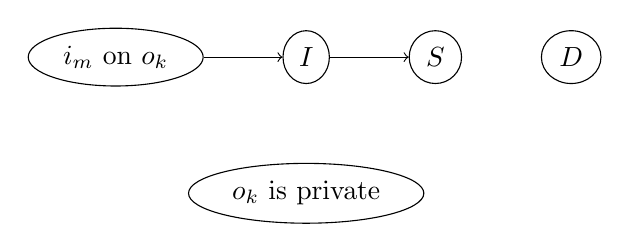
\begin{tikzpicture}[
        every node/.style={shape=ellipse, draw}
    ]
    %NODES
    %\node (mt) {$m \in t$};
    \node (io) {$i_{m}\textrm{ on }o_k$};
    \node (i)  [right = of io] {$I$};
    \node (s) [right = of i] {$S$};
    %\node (t) [below = of po, text width=2cm, align=center] {$i_m \textrm{ on } o_k, \exists i_l \textrm{ on } o_k$ s.t. $l \in t$};
    %\node (op) [below = of io] {$\exists i_l \textrm{ on } o_k \textrm{ s.t. } l \in t$};
    \node (or) [below = of i] {$o_k$ is private};
    \node (d) [right = of s] {$D$};

    %PATHS
    \path   (io) edge [->] (i);
    \path   (i) edge [->] (s);
    %\path   (po) edge [->] (t);
    %\path   (po) edge [->] node [left, draw=none] {$f_t$} (t);
    %\path   (or) edge [->] (op);
    \end{tikzpicture}
    \caption{Belief Network}\label{fig:belief}
    %\medskip
    %\small
\end{figure}

Now we are ready to perform some Bayesian inference to obtain $p(i_m \textrm{ on } o, o \textrm{ is private} \mid I, \textrm{ evidence})$.

\begin{align}
    & p(i_m \textrm{ on } o_k, o_k \textrm{ is priv} \mid I, \textrm{ evidence})     && = p(i_m \textrm{ on } o_k, o_k \textrm{ is priv} \mid I, S, D) \notag\\
    & \quad && = \frac
        {p(S, I, i_m \textrm{ on } o_k, o_k \textrm{ is priv}, D)}
        {p(S, I, D)} \notag\\
    & \quad && = \frac
        {p(S \mid I) p(I \mid i_m \textrm{ on } o_k) p(i_m \textrm{ on } o_k) p(o_k \textrm{ is priv}) p(D)}
        {p(S \mid I) p(I) p(D)} \notag\\
    & \quad && = \frac
        {p(I \mid i_m \textrm{ on } o_k) p(i_m \textrm{ on } o_k) p(o_k \textrm{ is priv})}
        {p(I)}\\
    & p(i_m \textrm{ on } o_k) 
        && = \sum\limits_{n \in \lbrack0,N)} \Big( p(I_n \mid i_m \textrm{ on } o_k) p(i_m \textrm{ on } o_k) \Big) \label{eqn:joint}\\
    & p(I)
        && = \sum\limits_{o_k \in O} \Big( p(I \mid i_m \textrm{ on } o_k) p(i_m \textrm{ on } o_k) \Big)%
\end{align}%

\subsubsection{Algorithm}

We will consider all the factors in Equation \ref{eqn:joint}.  $p(I \mid i_m \textrm{ on } o_k)$ is provided as noisy evidence, which has a high potential for resulting in a falsely high number of contiguous object regions.  Aside from the affect of identifying only small portions of private objects, this will also adversely affect $p(o_k \textrm{ is priv})$ by driving up the number of unmarked private objects and potentially mislabeling those that are marked.  Efficient belief propagation over pixels arranged as Markov Random Fields (MRF) has been shown to produce good results in scenarios where labels are unlikely to change between two neighboring pixels except in border regions \cite{felzenszwalb2006efficient}.  We use a variant of this approach to help regularize the noisy $p(I \mid i_m \textrm{ on } o_k)$ evidence to achieve $p_R(I \mid i_m \textrm{ on } o_k)$, as shown in Algorithm \ref{alg:regObjMap}.


\begin{algorithm}[h!]\label{alg:regObjMap}
\caption{Regularize the Object Map}
\KwData{
    $I: \lbrack 0,256 \rbrack^{M \times H} \rightarrow \{i_{mh} \mid \forall m \in \lbrack 0, M ), \forall h \in \lbrack 0, H)\}$
}
\KwResult{$p_R(I \mid i_m \textrm{ on } o_k)$}

$T \leftarrow$ small number // number of iterations for message updates\;
$d \leftarrow$ small positive constant // penalty for labeling variation\;
$D^{M \times K} \leftarrow -log(p(I \mid i_m \textrm{ on } o))$ /* get object probability map from noisy evidence and convert values to negative log */\;
MSG$^t \leftarrow 0^{M \times \lvert m\textrm{'s neighbors} \rvert \times K}$\;
MSG$^{t-1}$\;
res $\leftarrow$ null$^M$\;

\SetKwFunction{h}{h}
\SetKwProg{Def}{def}{:}{}
\Def{\h{x: coord}}{
    res $\leftarrow 0^K$\;
    \For{$k \leftarrow 0$ \KwTo $K$}{
        \For{$q \in$ Neighbors($x$)}{
            $res_k \leftarrow res_k +$ MSG$^{t-1}_{q,x,k}$\;
        }
        $res_k \leftarrow res_k + D_{x,k}$\;
    }
    return $res$
}

\SetKwFunction{Nei}{Neighbors}
\Def{\Nei{x}}{return 8 pixel coordinates around x // could be 4\;}

\For{$t \leftarrow 0$ \KwTo $T$}{
    // Update messages $T$ times\;
    MSG$^{t-1} \leftarrow$ MSG$^t$\;
    \For{$m \leftarrow 0$ \KwTo $M$}{
        // for each pixel coordinate\;
        $h_m \leftarrow$ \h{$m$}\;
        $h_{m_{min}} \leftarrow \min_{k} (h_m + d)$\;
        $Q \leftarrow$ Neighbors($m$)\;
        \For{$q \in Q$}{
            $h_q \leftarrow$ \h{$q$}\;
            \For{$k \leftarrow 0$ \KwTo $K$}{
                MSG$^t_{m,q,k} \leftarrow \min (h_{q_{k}}, h_{m_{min}})$
            }
        }
    }
}
\For{$m \leftarrow 0$ \KwTo $M$}{
    res$_m \leftarrow$ $\operatorname{arg\,min}_k$ \h{$m$}\;
}
return res\;
\end{algorithm}



There are three factors in Equation \ref{eqn:joint} which are not supplied by the evidence or known, and need to be found.  $p(o_k \textrm{ is priv})$ is the prior distribution for a given object type being private.  This distribution will need to be learned through an enumeration of object types and instances in all the images and tallying which types, and how many, have been marked private in our training data.

\begin{algorithm}
\KwData{this text}
\KwResult{this result}
\caption{hey there}
\end{algorithm}


\subsection{Task 2: Does the Image Contain Private Data?}

The objective for this task can be stated as estimating $p(C_I = 1 \mid I)$ where $C_I$ is the binary class label for whether the image is benign (0) or private (1).  


\subsubsection{Probabilistic Model Formulation}

Assuming there are $K$ objects in an image, if even one object in the image is private, then the image contains private content.  A simplistic approach might involve using the evidence $p(I_n \mid i_{nm} \textrm{ on } o)$ directly but, since it is noisy evidence, false positives are likely.  One would like to incorporate any and all useful evidence into the determination, and also reduce noise to achieve congruency for pixel-on-object predictions within object areas to reduce false positives. Therefore, a probabilistic model is needed.

When defining a probabilistic model, it is important to define the central assumptions behind what the model is attempting to capture in terms of privacy. For this approach, the following assumptions are used: (a) certain objects, or object details, are private, and (b) whether an image is private is determined by whether it contains private objects or object details.  Notice that certain contextual privacy scenarios, such as an image of a car known to belong to `Bob' being parked outside of a liquor store during work hours, for example, may not necessarily be marked private, even though `Bob' might argue that it is.

Under these assumptions, we can informally model the objective task as a set of Bernoulli trials over all objects in the image:

\begin{align}\label{eqn:task2.0}
    p(C_I = 1 \mid \textrm{evidence}) = 1 - \prod_{k \in K} \Big( 1 - p(\textrm{image region for $o_k$ is private} \mid \textrm{evidence}) \Big)
\end{align}

where $p(\textrm{image region for $o_k$ is private})$ is the marginal distribution of $o_k$ being object type $o$ and $o$ being a private type, as follows...

\begin{align}\label{eqn:task2.1}
    p(\textrm{image region for $o_k$ is private}) = \sum_{o \in O} p(o_k = o, o\textrm{ is private} \mid \textrm{evidence})    
\end{align}

\subsubsection{Basis of the Model}



Now we are ready to infer the marginal probability distribution for $p(\textrm{image region for $o_k$ is private}) = \sum_{o \in O} p(o_k = o, o\textrm{ is private} \mid \textrm{evidence})$.  First, solve for $p(o_k = o, o\textrm{ is private} \mid \textrm{evidence})$.

\begin{align*}
    p(o_k = o, o\textrm{ is private} \mid \textrm{evidence}) =
    %p((i_m \textrm{ on } o_k, \exists i_l \textrm{ on } o_k \textrm{ s.t. } l \in t) \mid o_k \textrm{ is private}, i_m \textrm{ on } o_k) p(o_k \textrm{ is private}) p(i_m \textrm{ on } o_k) p(I \mid i_m \textrm{ on } o_k) p(S \mid I) p(D)
    %p(I, S, D, i_{m} \textrm{ on } o,o \textrm{ is private}, t, Z_h) = & p(t \mid i_m \textrm{ on o}, o \textrm{ is private}, Z_h) \\
        %& p(i_m \textrm{ on o} \mid S, I) p(S \mid I) p(I) p(Z_h) p(o \textrm{ is private}) p(D)\\
\end{align*}

\subsubsection{Algorithm}

1. get joint prob map $p(i_{nm} \textrm{ on o}, S_n \mid I_n, t_n)$\\
2. use MRF (Felzenszwalb) to reduce noise \& increase congruence \cite{felzenszwalb2006efficient}.  Record max $o$ for segmentation.\\
3. use watershed segmentation to label objects (type \& instance) \cite{87344}. During algorithm, calculate average probability for each object instance (add all pixel probabilities and keep a queue pop counter for final division).  Also build dataset of object types \& instances and if $t_n=1$ is encountered, mark that instance private.  This will be used to build a distribution for $p(o \textrm{ is private}$\\
4. use \#3 to get $p(o_k = o)$\\
 




%%%%%%%%%%%%%%%%% BIB %%%%%%%%%%%%%%%%%%%%
\newpage
\bibliographystyle{plain}
\bibliography{references}
\addcontentsline{toc}{section}{References}


%%%%%%%%%%%%%%%%% Appendices %%%%%%%%%%%%%%%%%%%%
\newpage
\appendixtitleon
\begin{appendices}

\begin{center}
    \section{Examination Committee Questions}
\end{center}

\subsection{Dr. Apu Kapadia}

\subsubsection{GANs (2.5-3 pages excluding citations)}
Researchers have recently made much progress in the area of adversarial machine learning using "generative adversarial networks." Identify 8-12 papers in this area specific to computer vision, and synthesize and summarize the various research contributions in this area; draw connections between the various papers and make sure the writeup does NOT look like a string of summaries. Instead group and summarize categories and discuss how they relate to each other.  Make sure you critique the various works when you discuss them, discussing how these works address the weaknesses of the other works you discuss. 

Have a clearly marked section at the end (about 0.75 page) that talks about research challenges and directions forward from your perspective, i.e., what all remains to be done after your discussion of the various papers (including your own published work)?

\subsubsection{Adversarial machine learning (1.5-2 pages excluding citations)}
Model this section on the previous section, but expand the focus beyond computer vision and talk about 5-8 papers NOT related to computer vision and how machine learning algorithms can be 'tricked' by adversaries. Discuss how machine learning algorithms in the context of security can be made robust against adversaries trying to escape classification, for example.

\subsection{Dr. David Crandall}\label{app:crandall}


\subsection{Dr. Donald Williamson}

\end{appendices}

\end{document}
